\documentclass{article}
\usepackage{graphicx} % Required for inserting images
\usepackage[a4paper, margin=1in]{geometry}
\usepackage{amsmath}
\usepackage{authblk} 
\usepackage{tikz}

\title{Matrix Based SPH Formulation}
\author{Štěpán Müller}
\affil{Czech Technical University in Prague, Faculty of Mechanical Engineering}
\date{May 2024}

\begin{document}

\maketitle

\section{Introduction}
In this article, a matrix-based formulation of a numerical SPH scheme is presented. 
For demonstration, the following weakly compressible SPH scheme in 2 dimensions will be used:
$$\frac{D\rho_i}{Dt}=-\rho_i\sum_j\left(\textbf{u}_j-\textbf{u}_i\right)\cdot\nabla W_{ij}V_j+c_0\sum_j\left(\rho_j-\rho_i\right)\frac{\left(\textbf{r}_j-\textbf{r}_i\right)\cdot \nabla W_{ij}}{\mid\mid\left(\textbf{r}_j-\textbf{r}_i\right)\mid\mid^2}V_j$$

$$\frac{D\textbf{u}_i}{Dt}=-\frac{1}{\rho_i}\sum_j\left(p_j+p_i\right)\cdot\nabla W_{ij}V_j+\textbf{f}_i+\nu\frac{\rho_0}{\rho_i}\sum_j\pi_{ij}\nabla W_{ij}V_j$$

$$\frac{D\textbf{r}_i}{Dt}=\textbf{u}_i$$

$$p_i=c_0^2\left(\rho_i-\rho_0\right)$$

where $W_{ij}$ is the Gaussian Kernel, resulting in

$$\nabla W_{ij}= 
\begin{bmatrix}
x_j - x_i \\
y_j - y_i \\
\end{bmatrix}
\cdot\frac{2}{\pi h^4}\cdot exp\left(-\frac{\left(x_j-x_i\right)^2+\left(y_j-y_i\right)^2}{h^2}\right)$$

and $\pi_{ij}$ equals to
$$\pi_{ij}=8\cdot\frac{\left(\textbf{u}_j-\textbf{u}_i\right)\cdot\left(\textbf{r}_j-\textbf{r}_i\right)}{\mid\mid\textbf{r}_j-\textbf{r}_i\mid\mid^2}$$
A common algorithmization approach is to loop for $i$ over all particles and calculate their interactions with appropriate $j$ particles. The aim of the matrix based method presented in this article is to greatly reduce the amount of operations performed in a loop and replace them with matrix and vector operations.

\section{Constructing the matrix based formulation}
\subsection{Interaction matrix I}
The matrix method starts by identifying possible interacting particle pairs (for example using the bin sort method) and storing this information in the interaction matrix $I$. $I$ is a sparse square symetrical binary matrix of size $N\times N$, where $N$ is the number of particles.
$$I = 
\begin{bmatrix}
0 & 1 & 0\\
1 & 0 & 1\\
0 & 1 & 0\\
\end{bmatrix}
$$
Each row $i$ represents the interactions of particle $i$ with particles $j$, where $j$ is the column. Here the first row would mean that particle $1$ does not interact with itself, it interacts with particle $2$ and does not interact with particle $3$. 

$I$ can be stored for example in the COO sparse format. Finding the matrix $I$ is the only loop necessary to algorithmize the process.
\subsection{Vectors of variables}
The particle variables will be referred to as 1D vectors of length $N$, for example vector
$$
\vec{x}=
\begin{bmatrix}
x_1 & x_2 & x_3\\
\end{bmatrix}
$$
stores the $x$ coordinate of $N=3$ particles.
\subsection{Matrices of differences} \label{matrices of differences}
Matrices of differences will replace all members that involve $j-i$ subtraction, such as $x_j-x_i$.
At first a matrix $Mx$ is defined, which results from a column-wise multiplication of $\Vec{x}$ and $I$, such as
$$
Mx=
\begin{bmatrix}
x_1 & x_2 & x_3\\
\end{bmatrix}
\begin{bmatrix}
0 & 1 & 0\\
1 & 0 & 1\\
0 & 1 & 0\\
\end{bmatrix}
=
\begin{bmatrix}
0 & x_2 & 0\\
x_1 & 0 & x_3\\
0 & x_2 & 0\\
\end{bmatrix}
$$
The matrix of differences $Dx$ is defined:
$$
Dx=Mx-Mx^T=
\begin{bmatrix}
0 & x_2 & 0\\
x_1 & 0 & x_3\\
0 & x_2 & 0\\
\end{bmatrix}
-
\begin{bmatrix}
0 & x_1 & 0\\
x_2 & 0 & x_2\\
0 & x_3 & 0\\
\end{bmatrix}
=
\begin{bmatrix}
0 & x_2-x_1 & 0\\
x_1-x_2 & 0 & x_3-x_2\\
0 & x_2-x_3 & 0\\
\end{bmatrix}
$$
Using the same approach, difference matrices $Dy, Du, Dv, D\rho$ can be calculated, with the exception of difference matrix $Dp$, which uses addition instead of subtraction due to the chosen SPH scheme.

It requires emphasizing that all involved matrix by vector multiplications should utilize the sparsity of the matrix to prevent $O(N^2)$ time complexity, which would make all effort for further optimization entirely pointless.

\subsection{Matrix $\nabla W_x$ and $\nabla W_y$}
Hereafter, a simplified notation will be used:
$$ x_j-x_i=dx_{ij} $$
Steps to construct the $\nabla W$ matrices follow:
$$
Mr^2 = Dx^2 + Dy^2 = 
\begin{bmatrix}
0 & x_{12}^2 & 0\\
x_{21}^2 & 0 & x_{23}^2\\
0 & x_{32}^2 & 0\\
\end{bmatrix}
+
\begin{bmatrix}
0 & y_{12}^2 & 0\\
y_{21}^2 & 0 & y_{23}^2\\
0 & y_{32}^2 & 0\\
\end{bmatrix}
=
\begin{bmatrix}
0 & r_{12}^2 & 0\\
r_{21}^2 & 0 & r_{23}^2\\
0 & r_{32}^2 & 0\\
\end{bmatrix}
$$
Using the exponential function, only non-zero elements are taken into account:
$$
\nabla W_{size} = exp_{arg\neq0}\left(\frac{-1}{h^2}Mr^2\right)\cdot\frac{2}{\pi h^4}
$$
Eventually, matrices $\nabla W_x$ and $\nabla W_y$ can be acquired using element-wise multiplication:
$$
\nabla W_x = Dx\nabla W_{size} = 
\begin{bmatrix}
0 & \frac{2dx_{12}}{\pi h^4}\cdot exp\left(-\frac{dx_{12}^2+dy_{12}^2}{h^2}\right) & 0\\
\cdots & 0 & \cdots\\
0 & \cdots & 0\\
\end{bmatrix}
$$

$$
\nabla W_y = Dy\nabla W_{size} = 
\begin{bmatrix}
0 & \frac{2dy_{12}}{\pi h^4}\cdot exp\left(-\frac{dx_{12}^2+dy_{12}^2}{h^2}\right) & 0\\
\cdots & 0 & \cdots\\
0 & \cdots & 0\\
\end{bmatrix}
$$
\subsection{Matrix $\pi$}
Similarly to construction of $\nabla W$, a matrix $\pi$ can be constructed using element-wise multiplications:
$$\pi = 8\cdot\left(DuDx + DvDy\right)\cdot\frac{1}{Mr^2}$$
\section{Final matrix SPH scheme}
For the chosen SPH scheme, the matrix formulation gives:
$$
\overrightarrow{\frac{D\rho}{Dt}}=-\Vec{\rho}\left[\left(Du\nabla W_x + Dv \nabla W_y\right)\cdot\Vec{V}\right]
+
c_0\left[\frac{D\rho\left(Dx\nabla W_x + Dy\nabla W_y \right)}{\sqrt{Mr^2}}\right]\cdot\Vec{V}
$$
$$
\overrightarrow{\frac{Du}{Dt}}=\frac{-1}{\Vec{\rho}}\left[\left(Dp\nabla W_x\right)\cdot\Vec{V}\right]+\frac{\nu\rho_0}{\Vec{\rho}}\left[\left(\pi\nabla W_x\right)\cdot\Vec{V}\right]+\Vec{g_x}
$$
$$
\overrightarrow{\frac{Dv}{Dt}}=\frac{-1}{\Vec{\rho}}\left[\left(Dp\nabla W_y\right)\cdot\Vec{V}\right]+\frac{\nu\rho_0}{\Vec{\rho}}\left[\left(\pi\nabla W_y\right)\cdot\Vec{V}\right]+\Vec{g_y}
$$
$$\overrightarrow{\frac{Dx}{Dt}}=\Vec{u}$$
$$\overrightarrow{\frac{Dy}{Dt}}=\Vec{v}$$
$$
\vec{p}=c_0^2\left(\Vec{\rho}-\Vec{\rho_0}\right)
$$
where the $\cdot$ symbol indicates basic matrix by vector multiplication, whereas no dot suggests element-wise multiplication. 
\section{Data handling optimization}
\subsection{Data vector format}
Because matrices 
$$Dx, Dy, Du, Dv, Dp, Mr^2, \nabla W_{size}, \nabla W_x, \nabla W_y, \pi$$
all have the same structure, sharing the row and column indices of $I$, most operations can be only performed on the data vector using the COO matrix format. Using the example notation
$$\vec{Dx} = Dx.data$$
the scheme can be rewritten to a more efficient vector format. The only need to reuse the full matrix format comes from the $\cdot$ multiplication by vector of volumes $\Vec{V}$:

$$
\overrightarrow{\frac{D\rho}{Dt}}
=
-\Vec{\rho}\left[to\_coo\_matrix\left(\vec{Du}\vec{\nabla W_x} + \vec{Dv} \vec{\nabla W_y}\right)\cdot\Vec{V}\right]
+
to\_coo\_matrix\left[\frac{c_0 \Vec{D\rho}\left(\Vec{Dx}\Vec{\nabla W_x} + \Vec{Dy}\Vec{\nabla W_y} \right)}{\sqrt{\Vec{Mr^2}}}\right]\cdot\Vec{V}
$$
$$
\overrightarrow{\frac{Du}{Dt}}
=
\frac{1}{\Vec{\rho}}\left[to\_coo\_matrix\left(\vec{-Dp}\vec{\nabla W_x}+\nu\rho_0\vec{\pi}\vec{\nabla W_x}\right)\cdot\Vec{V}\right]+\Vec{g_x}
$$
$$
\overrightarrow{\frac{Dv}{Dt}}
=
\frac{1}{\Vec{\rho}}\left[to\_coo\_matrix\left(\vec{-Dp}\vec{\nabla W_y}+\nu\rho_0\vec{\pi}\vec{\nabla W_y}\right)\cdot\Vec{V}\right]+\Vec{g_y}
$$
\subsection{Simplified way to calculate data vectors}
Furthermore, there is a simplier way to calculate the difference data vectors $\Vec{Dx}, \Vec{Dy}, \Vec{Du}, \Vec{Dv}, \Vec{D\rho}, \Vec{Dp}$ by only using row and column vector of the sparse COO matrix $I$, instead of using full sparse multiplication:
$$\Vec{Dx} = \Vec{x}[columns]-\Vec{y}[rows] $$
Where $\Vec{x}[columns]$ means selecting $x_i$ so that $i$ goes through all column indices of $I$. Using $I$ from previous chapters as example:
$$I = 
\begin{bmatrix}
0 & 1 & 0\\
1 & 0 & 1\\
0 & 1 & 0\\
\end{bmatrix}
\to I.rows = 
\begin{bmatrix}
1 & 2 & 2 & 3\\
\end{bmatrix}
; I.columns = 
\begin{bmatrix}
2 & 1 & 3 & 2\\
\end{bmatrix}
; I.data = 
\begin{bmatrix}
1 & 1 & 1 & 1\\
\end{bmatrix}
$$
$$
\vec{x}=
\begin{bmatrix}
x_1 & x_2 & x_3\\
\end{bmatrix}
; 
\vec{x}[columns]=
\begin{bmatrix}
x_2 & x_1 & x_3 & x_2\\
\end{bmatrix}
; 
\vec{x}[rows]=
\begin{bmatrix}
x_1 & x_2 & x_2 & x_3\\
\end{bmatrix}
$$
$$
\Vec{Dx} = 
\begin{bmatrix}
x_2-x_1 & x_1-x_2 & x_3-x_2 & x_2-x_3\\
\end{bmatrix}
$$
As shown, this method provides the same result for $\Vec{Dx}$ as the method from \ref{matrices of differences}.

\section{Procedural modification of the interaction matrix}
In the previous chapters, it was shown how a full SPH calculation scheme can be built based on a single interaction matrix $I$. Every iteration it is firstly required to build $I$, as $I$ might be different every iteration due to the movement of interacting particles.

The most basic way to build $I$ is to use the bin sort algorithm and construct $I$ from scratch every iteration. This suggests to loop over the bins, which might not be performed as efficiently as the rest of the matrix-based algorithm. 

Therefore in this chapter, a different method of managing $I$ is presented.
\subsection{Standard bin sort method}
At first, let's look at the standard bin sort method of generating $I$ for a 2 dimensional case.

The bin sort method divides the XY coordinate space into bins and assigns a corresponding bin to every particle (or assigns a set of particles to every bin).

Let's consider 5 particles:
$$
\Vec{x} = 
\begin{bmatrix}
1 & 5 & 2 & 5 & 5\\
\end{bmatrix}
$$
$$
\Vec{y} = 
\begin{bmatrix}
1 & 2 & 5 & 5 & 8\\
\end{bmatrix}
$$
Let's sort them into 9 bins using the following labels:

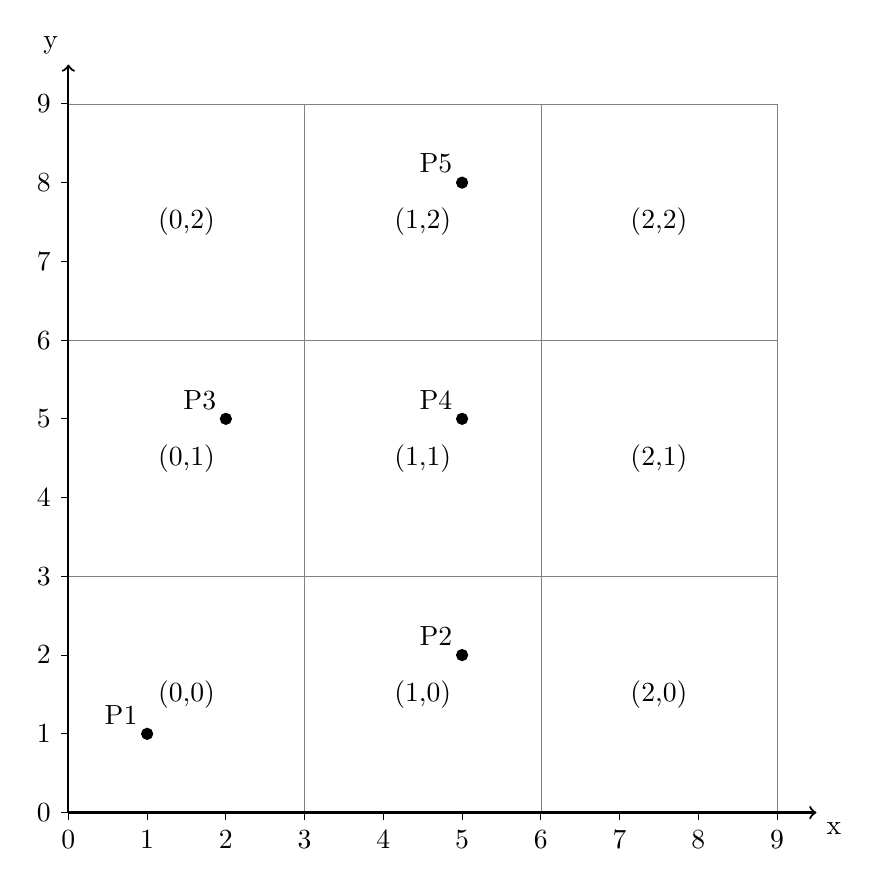
\begin{tikzpicture}
    % Draw the grid
    \draw[step=3cm,gray,very thin] (0,0) grid (9,9);

    % Draw the axes
    \draw[thick,->] (0,0) -- (9.5,0) node[anchor=north west] {x};
    \draw[thick,->] (0,0) -- (0,9.5) node[anchor=south east] {y};

    % Label the axes
    \foreach \x in {0,1,...,9}
        \draw (\x,0) -- (\x,-0.1) node[anchor=north] {\x};
    \foreach \y in {0,1,...,9}
        \draw (0,\y) -- (-0.1,\y) node[anchor=east] {\y};

    % Draw the sector coordinates
    \foreach \x in {0,1,2}
        \foreach \y in {0,1,2}
            \node at (\x*3+1.5,\y*3+1.5) {(\x,\y)};

    % Draw the points
    \filldraw[black] (1,1) circle (2pt) node[anchor=south east] {P1};
    \filldraw[black] (5,2) circle (2pt) node[anchor=south east] {P2};
    \filldraw[black] (2,5) circle (2pt) node[anchor=south east] {P3};
    \filldraw[black] (5,5) circle (2pt) node[anchor=south east] {P4};
    \filldraw[black] (5,8) circle (2pt) node[anchor=south east] {P5};

\end{tikzpicture}

The information about where each point belongs can be represented as:
$$
\Vec{binx} = 
\begin{bmatrix}
0 & 1 & 0 & 1 & 1\\
\end{bmatrix}
$$
$$
\Vec{biny} = 
\begin{bmatrix}
1 & 2 & 1 & 1 & 2\\
\end{bmatrix}
$$
Looping over all bins and browsing adjacent bins for interacting particles gives $I$:
$$
I = 
\begin{bmatrix}
0 & 1 & 1 & 1 & 0\\
1 & 0 & 1 & 1 & 0\\
1 & 1 & 0 & 1 & 1\\
1 & 1 & 1 & 0 & 1\\
0 & 0 & 1 & 1 & 0\\
\end{bmatrix}
$$

\subsection{Prerequisites of the procedural modification method}
The following method of generating $I$ is based on the prerequisite, that $I$ usually changes only very slightly between each iteration. 

Let there be $N$ particles distributed approximately evenly with an average spacing $s$. The weighting length $h$ can be chosen as for example $1.5S$. Consequently, when using the Gaussian kernel, the size of one bin is $3S=2h$. The simulation runs with a constant timestep $T$ and particles have an average velocity of $u$.

Under these circumstances, the average number of particles that leave their bin during one iteration will be on the order of
$$
N_{bin\ changes}\approx N \cdot \frac{u \cdot T}{3S} = N \cdot \frac{u \cdot T}{2h} 
$$
The timestep $T$ can be derived from the CFL condition (missing reference):
$$
T = \alpha \cdot \frac{2h}{c}
$$
where $c$ is velocity of sound and $\alpha$ can be set constant to $0.4$ according to (reference).
Substituting for $T$ in the first equation:
$$
N_{bin\ changes}\approx N \cdot \frac{u \cdot 0.4\cdot \frac{2h}{c}}{2h} = N \cdot \frac{0.4u}{c}= N \cdot 0.4Ma
$$
For water flowing at $10 m/s$:
$$
N_{bin\ changes}\approx N \cdot \frac{0.4\cdot 10}{1500}\approx 3\cdot 10^{-3} N
$$
As shown, the number of bin changes per iteration will generally be much lower than number of particles. 
The goal of the following method is to utilize this and avoid generating brand new $I$ every iteration.
\subsection{Procedural modification method}
Let's assume that the $I_{k-1}$ was created in the previous iteration $k-1$. 
It is also known which bins were occupied in the previous iteration:
$$
Iteration\  k-1:
$$
\begin{minipage}[t]{0.3\textwidth}
    \vspace{0pt} % This ensures the top alignment
    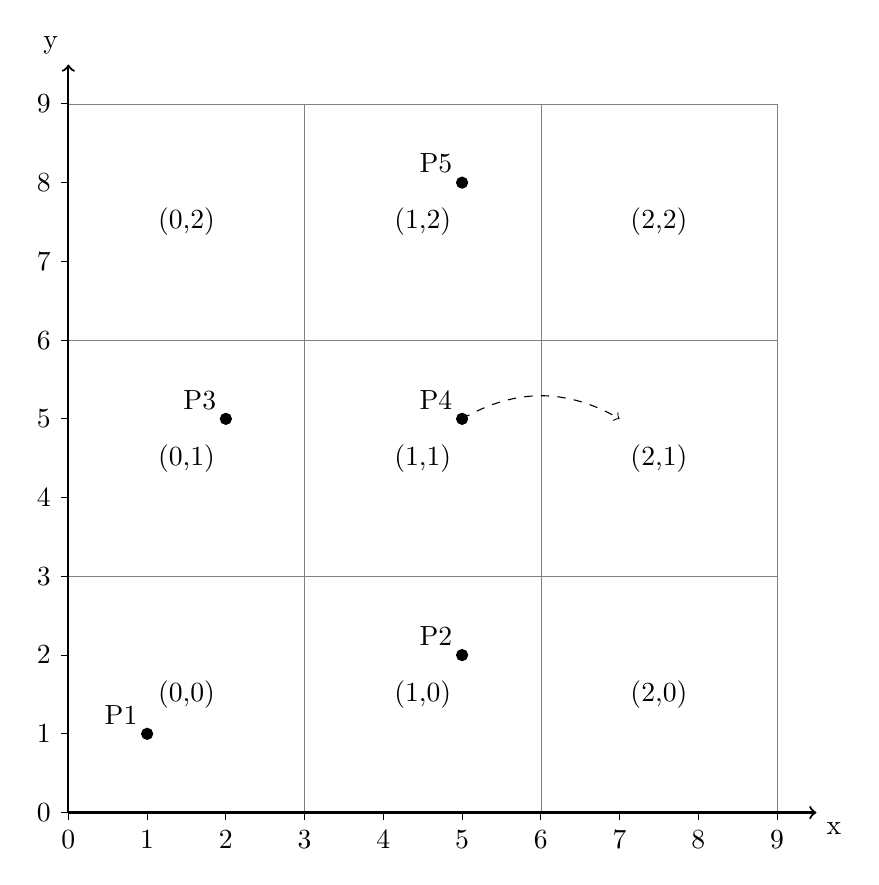
\begin{tikzpicture}
        % Draw the grid
        \draw[step=3cm,gray,very thin] (0,0) grid (9,9);

        % Draw the axes
        \draw[thick,->] (0,0) -- (9.5,0) node[anchor=north west] {x};
        \draw[thick,->] (0,0) -- (0,9.5) node[anchor=south east] {y};

        % Label the axes
        \foreach \x in {0,1,...,9}
            \draw (\x,0) -- (\x,-0.1) node[anchor=north] {\x};
        \foreach \y in {0,1,...,9}
            \draw (0,\y) -- (-0.1,\y) node[anchor=east] {\y};

        % Draw the sector coordinates
        \foreach \x in {0,1,2}
            \foreach \y in {0,1,2}
                \node at (\x*3+1.5,\y*3+1.5) {(\x,\y)};

        % Draw the points
        \filldraw[black] (1,1) circle (2pt) node[anchor=south east] {P1};
        \filldraw[black] (5,2) circle (2pt) node[anchor=south east] {P2};
        \filldraw[black] (2,5) circle (2pt) node[anchor=south east] {P3};
        \filldraw[black] (5,5) circle (2pt) node[anchor=south east] {P4};
        \filldraw[black] (5,8) circle (2pt) node[anchor=south east] {P5};
        % Draw the dashed curved arrow
        \draw[dashed, ->] (5,5) to[bend left] (7,5);
    \end{tikzpicture}
\end{minipage}
\begin{minipage}[t]{0.95\textwidth}
    \vspace{75pt} % This ensures the top alignment
    % Display the vectors
    \[
    \Vec{x_{k-1}} = 
    \begin{bmatrix}
    1 & 5 & 2 & 5 & 5\\
    \end{bmatrix}
    \]
    \[
    \Vec{y_{k-1}} = 
    \begin{bmatrix}
    1 & 2 & 5 & 5 & 8\\
    \end{bmatrix}
    \]
    \[
    \Vec{binx_{k-1}} = 
    \begin{bmatrix}
    0 & 1 & 0 & 1 & 1\\
    \end{bmatrix}
    \]
    \[
    \Vec{biny_{k-1}} = 
    \begin{bmatrix}
    1 & 2 & 1 & 1 & 2\\
    \end{bmatrix}
    \]
    
    \[
    I_{k-1} = 
    \begin{bmatrix}
    0 & 1 & 1 & 1 & 0\\
    1 & 0 & 1 & 1 & 0\\
    1 & 1 & 0 & 1 & 1\\
    1 & 1 & 1 & 0 & 1\\
    0 & 0 & 1 & 1 & 0\\
    \end{bmatrix}
    \]
\end{minipage}

In the next iteration $k$, the particle $P4$ moves from $[5\  5]$ to $[7\  5]$, which shifts it to a different bin. The new bin vectors can be calculated by dividing coordinate vectors by bin size $2h = 3$ and ceiling them to the closest lower integer:
$$
\Vec{x_{k}} = 
\begin{bmatrix}
    1 & 5 & 2 & 7 & 5\\
\end{bmatrix}
$$
$$
\Vec{y_{k}} = 
\begin{bmatrix}
    1 & 2 & 5 & 5 & 8\\
\end{bmatrix}
$$
$$
\Vec{binx_{k}} = ceil\left(\frac{\Vec{x_{k}}}{2h}\right)=
\begin{bmatrix}
    0 & 1 & 0 & 2 & 1\\
\end{bmatrix}
$$
$$
\Vec{biny_{k}} = ceil\left(\frac{\Vec{y_{k}}}{2h}\right)=
\begin{bmatrix}
    1 & 2 & 1 & 1 & 2\\
\end{bmatrix}
$$
The new and old bin vectors can be subtracted:
$$
\Vec{Dbinx} = \Vec{binx_{k}} - \Vec{binx_{k-1}}=
\begin{bmatrix}
    0 & 1 & 0 & 2 & 1\\
\end{bmatrix}
-
\begin{bmatrix}
    0 & 1 & 0 & 1 & 1\\
\end{bmatrix}
=
\begin{bmatrix}
    0 & 0 & 0 & 1 & 0\\
\end{bmatrix}
$$
$$
\Vec{Dbiny} = \Vec{biny_{k}} - \Vec{biny_{k-1}}=
\begin{bmatrix}
    1 & 2 & 1 & 1 & 2\\
\end{bmatrix}
-
\begin{bmatrix}
    1 & 2 & 1 & 1 & 2\\
\end{bmatrix}
=
\begin{bmatrix}
    0 & 0 & 0 & 0 & 0\\
\end{bmatrix}
$$
Absolute values of $\Vec{Dbinx}$ and $\Vec{Dbiny}$ can be added to identify which particles left their bin whichever direction. The resulting sparse vector should be clipped to 1 from the top to allow further operations:
$$
\Vec{Dbin} = clip(\mid\Vec{Dbinx}\mid + \mid\Vec{Dbiny}\mid) =  
\begin{bmatrix}
    0 & 0 & 0 & 1 & 0\\
\end{bmatrix}
$$
Now, all interactions of particle 4 need to be removed from $I_{k-1}$ to get $I_{cleaned}$ which no longer contains any outdated interactions. This can be done by subtracting two matrices from $I$, which result from column and row multiplication of $I$ by $\Vec{Dbin}$:
$$
I_{cleaned}=I_{k-1}-\Vec{Dbin}I-\Vec{Dbin}^TI=
$$
$$
=
\begin{bmatrix}
    0 & 1 & 1 & 1 & 0\\
    1 & 0 & 1 & 1 & 0\\
    1 & 1 & 0 & 1 & 1\\
    1 & 1 & 1 & 0 & 1\\
    0 & 0 & 1 & 1 & 0\\
\end{bmatrix}
-
\begin{bmatrix}
    0 & 0 & 0 & 1 & 0\\
\end{bmatrix}
\begin{bmatrix}
    0 & 1 & 1 & 1 & 0\\
    1 & 0 & 1 & 1 & 0\\
    1 & 1 & 0 & 1 & 1\\
    1 & 1 & 1 & 0 & 1\\
    0 & 0 & 1 & 1 & 0\\
\end{bmatrix}
-
\begin{bmatrix}
    0\\
    0\\
    0\\
    1\\
    0\\
\end{bmatrix}
\begin{bmatrix}
    0 & 1 & 1 & 1 & 0\\
    1 & 0 & 1 & 1 & 0\\
    1 & 1 & 0 & 1 & 1\\
    1 & 1 & 1 & 0 & 1\\
    0 & 0 & 1 & 1 & 0\\
\end{bmatrix}
=
$$
$$
=
\begin{bmatrix}
    0 & 1 & 1 & 1 & 0\\
    1 & 0 & 1 & 1 & 0\\
    1 & 1 & 0 & 1 & 1\\
    1 & 1 & 1 & 0 & 1\\
    0 & 0 & 1 & 1 & 0\\
\end{bmatrix}
-
\begin{bmatrix}
    0 & 0 & 0 & 1 & 0\\
    0 & 0 & 0 & 1 & 0\\
    0 & 0 & 0 & 1 & 0\\
    0 & 0 & 0 & 0 & 0\\
    0 & 0 & 0 & 1 & 0\\
\end{bmatrix}
-
\begin{bmatrix}
    0 & 0 & 0 & 0 & 0\\
    0 & 0 & 0 & 0 & 0\\
    0 & 0 & 0 & 0 & 0\\
    1 & 1 & 1 & 0 & 1\\
    0 & 0 & 0 & 0 & 0\\
\end{bmatrix}
=
$$
$$
=
\begin{bmatrix}
    0 & 1 & 1 & 0 & 0\\
    1 & 0 & 1 & 0 & 0\\
    1 & 1 & 0 & 0 & 1\\
    0 & 0 & 0 & 0 & 0\\
    0 & 0 & 1 & 0 & 0\\
\end{bmatrix}
$$
All interactions of particle 4 are now cleared up. Next step is to replace them with new interactions.
\section{Note about performance}
Compared to the standard looping method, which only requires to store vectors as long as $N$, the matrix based method requires to write vectors of length equal to number of particle pairs. Length of those vectors might range on the order of $10N$ to $100N$.

Despite the memory downside, removing most of the iterative loop using the matrix formulation could provide advantages in cases where memory is not the limit, and computational speed has the highest priority. Implementing the matrix method using efficient multiprocessing for matrix/vector operations needs to be investigated in order to evaluate practical benefits.
\section{Conclusion}
A matrix based formulation of a chosen SPH scheme was discussed. The principle of the matrix method was explained. A final matrix SPH scheme was derived. Two ways for optimization of the algorithm were shown. Expected performance of the method was briefly discussed. More research and practical implementation is expected to be necessary for proper evaluation.
\end{document}
